\section{Preventive Measures} \label{sec: preventive measure}

It is impossible to debate the spread of COVID-19 without including the numerous and different preventive measures that have been implemented both internationally and nationally. As COVID-19 can be a potentially catastrophic, global event if no global preventive or mitigative measures are implemented, it is also relevant to outline several types of preventive measures. Some preventive measures can be implemented by an individual or a group of individuals. Others are implemented by an authority like a government.

We aim to use our model to compare and contrast different preventive and mitigative measures when simulating COVID-19. Therefore, a comprehensive outlining of the many preventive measures that have been implemented within Denmark is needed. In this section, we will outline many different factors that aid prevention of COVID-19, with the goal of implementing variables with adjustable parameters into the simulation, which are relevant and plausible. While all the mentioned preventive measures might not be used for the final simulation, this will make it possible to argument, as to why we might leave some of these measures out.

\subsection{The Insecurity of Social Responsibility}

At the core of any preventive measure that spans around an entire society, whether local, regional or even global, is of course individual, social responsibility. In short, it is always up to the individual to adhere to the rules put in place by the relevant authorities, and if no rules are being forced, some form of social responsibility is still expected. A comprehensive overview of mitigative measures that can be implemented by the individual is found in \textit{COVID-19 (SARS-CoV-2) pandemic: fears, facts and preventive measures} \citep{ayenigbara_covid-19_2020}, who have also created figure \ref{fig:Mitigative-Measures}. These mitigative measures all stem from the basic principle of the individual’s own will to comply with them. Therefore, many of the preventive and mitigative measures mentioned in this report will be based - at least in part - on this figure.

\begin{figure}[H]
    \centering
    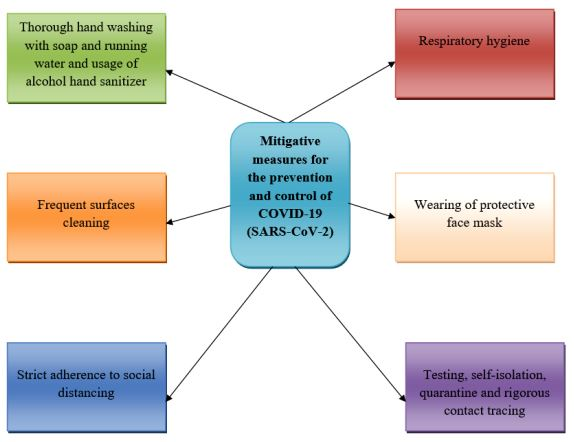
\includegraphics[width=0.75\textwidth]{0_billeder/mitigation of COVID-19.JPG}
    \caption{Mitigative measures that should be implemented across a society to combat COVID-19 \citep{ayenigbara_covid-19_2020}}
    \label{fig:Mitigative-Measures}
\end{figure}

Here, a note of definitions must be made. The word "mitigative" does of course not have the same definition as the word "preventive". Mitigative actions are not, per se, actions that can completely prevent the transmission of COVID-19, but rather to minimize the risk of rampant the spread. When discussing an illness like COVID-19, a realistic and critical view of the situation is important, and unfortunately, it is more realistic to focus on both mitigative and preventive measures, than purely on preventive measures.

As social responsibility relies heavily on every single individual in a given, geographical location, this parameter must be considered relatively insecure in nature. Therefore, social responsibility as a factor has been parted into the following multiple parameters to ensure minimal insecurity for each factor, and to ensure a way to quantify these factors. 

\subsection{Hygiene}
As shown in figure \ref{fig:Mitigative-Measures}, hygienic prevention is key for the individual to prevent spread of COVID-19 and ensure the safety of both themselves and others. Four of the six mentioned mitigative measures relates to personal hygiene or cleanliness of the environment (hand-washing, respiratory hygiene, mask-wearing, and surface-cleaning). For this report, we will consider respiratory hygiene measures as an umbrella term underneath, in which mask-wearing is the main component.

\subsubsection{Mask-wearing}
A popular means of prevention against COVID-19 amongst civilians and medical personnel alike, has been the usage of face masks- and shields. Ayenigbara et al. defines a protective face mask as a mask made of ``protective materials used to cover the nose and mouth in order to prevent the spread of highly infectious respiratory deseases like influenza, MERS and COVID-19.''\citep{ayenigbara_covid-19_2020}. Wearing protective face masks are particularly helpful in minimizing the risk of transmission via droplets, one of two main methods by which the virus spreads (The other being via touching surfaces).

Wearing masks is particularly useful in minimizing the spread, from persons who have tested positive to other persons \citep{ayenigbara_covid-19_2020}. It should be noted that wearing a mask whilst uninfected, will also still reduce the risk of transmission, though it seems rather impossible to quantity this. In short, wearing a mask both mitigates the general spread and the individual's risk of infection.

\textbf{Other Respiratory Hygiene Measures}
Other than mask-wearing, other respiratory hygiene measures can also mitigate spread of COVID-19. One such example of respiratory hygiene is sneezing and coughing into something that can preferably be immediately disposed of, such as tissue paper. 

Generally speaking, minimizing the transmission of droplets or aerosols via sneezing and coughing, helps mitigate the spread of COVID-19. The status of the virus cannot be seen as being airborne, though it cannot be ruled out, that it can spread via aerosols, as an example in ambient air. Therefore it is also of great importance to have efficient ventilation in the room you are present in. For this report we won't consider COVID-19 as being airborne, as it mainly spreads via droplets, and presumably in rare cases it can spread via aerosols in ambient air, if the ventilation is poor.


\subsection{Hand Sanitiser and Other Hygienic Measures}
While COVID-19 mainly spreads through droplets, it can also be transmitted via physical touching of surfaces or substances (and persons) that have been exposed to COVID-19. The risk of infection is highest if the eyes, nose and/or mouth is in contact with a surface, substance or person that is in contact or has been in contact with the virulent pathogen known as Sars-Cov-2 \citep{ayenigbara_covid-19_2020}. As explained in subsection \ref{sub:virology} - Virology of Sars-Cov-2, Sars-Cov-2 is the pathogen that leads to the illness known as COVID-19 or, in layman's terms, coronavirus.

Since Sars-Cov-2 is a highly contagious pathogen, it is important to maintain a high level of personal hygiene as well as hygiene in one's surroundings to minimize the risk of transmitting COVID-19. One obvious instance is through the rigorous usage of hand sanitizer and frequent hand-washing. To be at all effective, a hand sanitizer must be alcohol-based and properly and safely stored \citep{gharpure_knowledge_2020}.

While washing hands is a more thorough (if done correctly) way of preventing transmission of COVID-19, it can also be quite harsh on the skin to frequently use soap and similar cleaners - not to mention improbable in larger, semi-public areas such as supermarkets, schools and corporate workspaces according to \cite{cavanagh_rational_2020}. Therefore, hand sanitizer is the default "on-the-go" method for cleaning hands and thereby minimizing transmission through touching of surfaces. Lastly, each person should aim to touch their face as little as possible throughout their day. This measure will also aid in minimizing risk of infection via one's own mask.

\subsection{Social Distancing and Quarantine}
A parametre that is almost completely up to each individual is social distancing. Social distancing is very simply put the act of keeping a physical distance to other people whilst in public and semi-public scenarios \citep{ayenigbara_covid-19_2020}. Social distancing should be corrected to physical distancing, as social distancing would mean to take distance from all social interactions, and not just try to limit the physical interaction with other people. This would in theory mean to refrain from even meeting and socializing online, which does not make sense in form of stopping or slowing down the transmission rate of COVID-19. Physical distancing in layman's terms is better known as social distancing, so we will be using that term for the remainder of this report. Social distancing can be differentiated from quarantine and lock down, by distinguishing social distancing as preventive on a smaller scale; each person must make an effort to distance themselves from each other. Inversely, quarantine is the act of self-isolating either individually or as a household.

Measures can be taken to ensure minimal distance between two persons who, for instance, need to be closer than 2 metres to interact in relation to the exchange of goods and services. The usage of see-through plastic barriers between cashiers and customers in retail shops is one such example, where minimal distance is ensured without interfering with the experience. However, for most instances, social distancing should be considered the primary, preventive measure.

\textbf{Quarantine or Self-Isolation}

Quarantine is not a preventive measure if we assume what is to be prevented is illness. However, when it comes to a pandemic, society as a whole must aim to prevent further spread of the illness in question. Quarantine is a state of living that a person enters once they have been infected with the illness, or suspects they've become infected - in this case COVID-19. Quarantine can hereby become a preventive measure on a larger scale; when sectioning off persons infected with COVID-19, you prevent further transmission to others. During the international COVID-19 crisis, the word "self-isolation" has also been used to explain this state of living. In this report and context, the two terms are considered synonymous, regardless of etymological differences and historical applications.

As opposed to social distance, once a person has entered quarantine, they are not to interact with anyone – including within their own household. If the layout of the home permits it, they should stay completely separate from the rest of the people living with them, and cleaning should be a higher priority to ensure minimal risk of spreading via surfaces (furniture and the like) \citep{ayenigbara_covid-19_2020}. Regardless of whether a person is self-isolating by themselves or their family, the point is to mitigate contact with other people.

\subsection{Assembly Ban and Lockdown}

Although both assembly bans and lock downs can be considered part of social distance, there are some defining, differing factors. Firstly, an assembly ban or lock down is simply the governmentally implemented ban on assemblies (meaning social groups) that exceed a certain number. For instance, in March 2020, assemblies exceeding 100 people were banned by the government in Denmark \citep{ronnstad_tidslinje_2020}. This came hand in hand with the first national lock down of Denmark, in the early stages of the transmission of COVID-19 in northern Europe. 

\textbf{Assembly Ban}

Banning larger gatherings and social assemblies does not target specific social groups, religious groups or political groups when it is done as a preventive measure against pandemics. As such, while assembly bans can normally be quite polarising and controversial, they have been largely accepted by the general public across the world \citep{gostin_governmental_2020}. 

Assembly bans can, as mentioned, be given a quantifier in the form of an upper limit of individuals in a given group. This quantifier is chosen by the relevant authorities, which are Statens Serum Institut\citep{ssi_statens_nodate}, the Danish Government and the Danish Health Authority in Denmark's case. 

In March 2020, an assembly ban was introduced to Denmark. In the following five months, the assembly ban fluctuated between a maximum of 1,000 people to a maximum of just 10 people. As of the 23rd of October 2020, following a second wave of COVID-19 infections in the country, Denmark has a temporary assembly ban of 10 people or more \citep{ronnstad_tidslinje_2020}.

\textbf{Nationwide Lockdown}

Several nations have found it necessary to implement nationwide lock downs to combat the spread of COVID-19. China, Italy and the state of New York in the United States of America have all used some kind of lock down to mitigate the virus spreading. The effects of these lock downs can be seen in figure \ref{fig:Confirmed-infections-international} of confirmed infections \citep{zhang_identifying_2020}.

\begin{figure}[H]
    \centering
    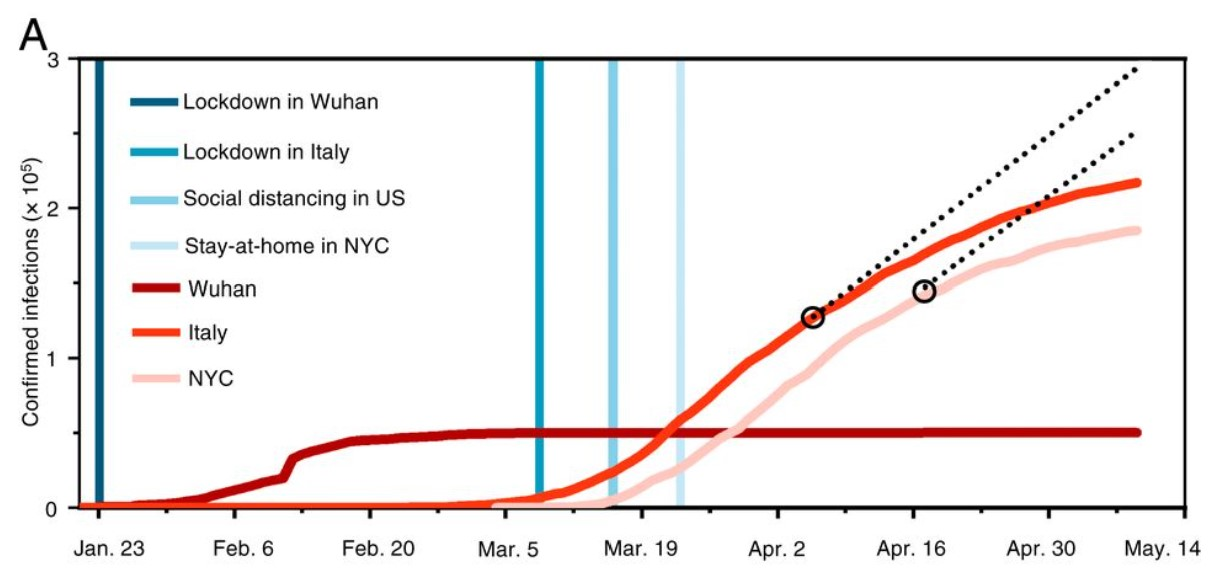
\includegraphics[width=\textwidth]{0_billeder/confirmed-infections-international.jpg}   
    \caption{Comparison of infection trends between Wuhan province, New York State and Italy including when lock down and similar preventive measures were implemented.
    \citep{zhang_identifying_2020}}
    \label{fig:Confirmed-infections-international}
\end{figure}

As shown in figure \ref{fig:Confirmed-infections-international}, the steady increase in confirmed infections was curbed after implementing either a temporary lock down, stay-at-home orders or social distancing. Lock downs can be considered the most serious implementation of what is, at its core, a form of social distancing. 

When a lock down is implemented, schools and non-essential businesses are typically closed and assembly bans are implemented. Depending on severity of the infection rate, stay-at-home orders and curfews can also be implemented. Lastly, quarantines for inbound travelers or actual bans on inbound travelling can also be implemented as part of nationwide lock down \citep{gostin_governmental_2020}.

\subsection{Information and Misinformation}

General information given to both the general public and lesser authorities within a society regarding COVID-19 is one of the most effective ways to minimize further spread of the illness. Although misinformation is of course not a preventive measure, it is a large enough factor within prevention of COVID-19 to warrant a few words on the topic. In the modern day, a lot of information can be given to the general public digitally, such as through apps and websites. This will be further outlined in subchapter \ref{Contact Tracing}.

Bierwiaczonek, Kunst and Pich have already concluded that conspiracy theories surrounding COVID-19 reduces social distancing \citep{bierwiaczonek_belief_nodate}, and Tasnim et.al have similarly concluded that the general spread of misinformation hinder the mitigation of COVID-19 on both a local and global scale \citep{tasnim_impact_2020}. Lastly, Pennycook et.al. have paid special attention to how this misinformation especially spreads on social media (Facebook, Reddit, YouTube and the like) \citep{pennycook_fighting_2020}. It can therefore confidently be stated that misinformation can be detrimental to the general prevention of COVID-19 and similar, respiratory infections.

\textbf{Trust in Authority}

The World Health Organisation (WHO) is a major authority on COVID-19 and similar health topics that span the globe \citep{who_home_nodate}. WHO collects data about transmission, recovery rates, morbidity, and the like. They also inform the general, international public about precautionary measures each individual can make use of to minimize risk of infection for both themselves and their family. 

For Denmark specifically, Statens Serum Institut (SSI) is another authority. SSI is an institute that operates under the Danish Ministry of Health. SSI is one of the main sources this paper have used to collect raw data from, such as transmission and day-by-day development of the virus’ spread within the country \citep{ssi_statens_nodate}.
